\documentclass{beamer}
\usepackage[utf8]{inputenc}
\usepackage[frenchb]{babel}
\usepackage[T1]{fontenc}
\usepackage{graphics}
\usepackage{framed}
\usepackage{graphicx}
\usepackage{grffile}
\usepackage{longtable}
\usepackage{wrapfig}
\usepackage{rotating}
\usepackage[normalem]{ulem}
\usepackage{amsmath}
\usepackage{textcomp}
\usepackage{amssymb}
\usepackage{capt-of}
\usetheme{Madrid}

\title[Support pour Verificarlo]{Support de MPI/OpenMP et de la vectorisation dans Verificarlo}
\subtitle{Master Calcul Haute Performance et Simulation}

\author[Hery, Ali, Nicolas]{Hery ANDRIANANTENAINA \\ Ali LAKBAL \\ Nicolas BOUTON}

\institute[]{\textbf{Encadrant:} Eric PETIT}

\date{Année 2020-2021}

\begin{document}

\maketitle

\begin{frame}{Verificarlo}
    \begin{block}{Compilateur de base pour verificarlo}
      \begin{itemize}
          \item CLANG
          \item LLVM
      \end{itemize}
    \end{block}
  \begin{block}{Domaine d'utilisation de verificarlo}
    Verificarlo permet par instrumentation des opérations flottantes, de pouvoir déboguer les erreurs, dû à la précision machine.
  \end{block}
  \begin{block}{Vectorisation dans le calcul scientifique}
    Jeux d'instruction 
        \begin{itemize}
            \item 128 = sse
            \item 256 = avx
            \item 512 = avx512
        \end{itemize}
  \end{block}
\end{frame}

\begin{frame}{Verificarlo}
    \begin{block}{Compilation}
      \begin{figure}
          \centering
          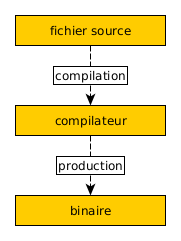
\includegraphics[width=6cm,height=4cm]{../ressources/compilation.png}
          \caption{Fonctionnement de base d'un compilateur}
          \label{fig:my_label}
      \end{figure}
    \end{block}
\end{frame}

\begin{frame}{Verificarlo}
    \begin{block}{Compilation pour verificarlo}
      \begin{figure}
          \centering
          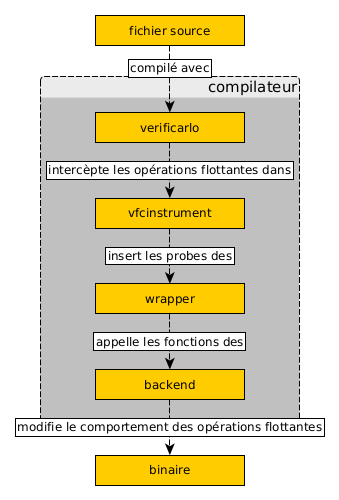
\includegraphics[width=6cm,height=6cm]{../ressources/verificarlo_works.png}
          \caption{Fonctionnement de verificarlo}
          \label{fig:my_label}
      \end{figure}
    \end{block}
\end{frame}

\begin{frame}{Définition de certains termes techniques}
      \begin{itemize}
          \item probes : Les probes sont des fonctions implémenté dans vfcwrapper qui est linker avec le programme par la partie compilation de verificarlo.
          \item backend : Dans le cadre de verifcarlo, c’est la/les librairie(s) dynamique(s) qui seront appelées par le wrapper dans les probes. Dans le cadre d’un compilateur c’est la derniere phase qui descend de la représentation intermédiaire vers le binaires
          \item wrapper : Ce sont des fonctions qui enveloppent l’appel à d’autres fonctions.
          \item link : Il s’agit de la phase de compilation qui consiste à aller chercher toute les librairies externes appelé par l’application pour les liées au programme utilisateur afin de résoudre les références non défini.
          \item sérialisation : Dans le contexte de l’utilisation de vecteur il s’agit d’exécuter en séquence les éléments du vecteur.
      \end{itemize}
\end{frame}

\begin{frame}{Support MPI/openMP}
    \begin{block}{Notion indispensable pour le parallélisme}
      \begin{itemize}
          \item Système à mémoire partage
            \begin{itemize}
                \item SMP
                \item NUMA
            \end{itemize}
          \item Système à mémoire distribuée
          \item Thread ou flot d'exécution
          \item Processus
          \item Calcul parallèle
      \end{itemize}
    \end{block}
    
    \begin{block}{Présentation d'open MPI}
      \begin{itemize}
          \item Installation : source: https://www.open-mpi.org/software/ompi/v4.1/
          \item Configuration : ./configure --prefix='/chemin/bin'
          \item Compilation : \textbf{make}
          \item Installation : \textbf{sudo make install}
          \item Préparation de l'environnement : 
      \end{itemize}
    \end{block}
\end{frame}

\begin{frame}{Présentation d'open MPI}
    \begin{block}{Description de communication dans Open MPI}
      \begin{itemize}
          \item l’environnement d’exécution
          \item les communication point à point
          \item les communication collectives
          \item les groupes de processus
          \item les topologies de processus
      \end{itemize}
    \end{block}
    
    \begin{block}{Compilation d’un programme parallèle avec verificarlo}
      \textbf{CC=OMPI\_CC=verificarlo mpicc}
    \end{block}
    \begin{block}{Bibliography}
        \begin{itemize}
            \item https://www.open-mpi.org
            \item https://fr.wikibooks.org
        \end{itemize}      
    \end{block}
\end{frame}

\begin{frame}{Vectorisation}
\begin{block}{Introduction }
    \begin{itemize}
        \item \textbf{Compilateurs:} \textit{ Clang et gcc} 
        \item \textbf{probleme:} \textit{  le support de
gcc était éphémère dû à une dépendance avec fortran qui vas étre enlevé dans le futur}
         \item \textbf{solutions : } \textit{supporter les types vectoriels de \textbf{clang} }
         \item \textbf{test: } \textit{ configurer \textbf{verificarlo} avec \textbf {clang} pour le C et C++ avec la commande suivante : }
         \end{itemize}
         \begin{center}
        \textbf{\color{blue} ./configure --without-flang CC=clang CXX=clang++ }      
          \end{center}
  \end{block}
\end{frame}

\begin{frame}{Vectorisation}
\begin{block}{Tests}
    \begin{itemize}
        \item\textit{ Suivre le fonctionnement de test que
Verificarlo a commencé à implémenter. } 
         \item \textit{Les tests sont principalement écrient en bash, avec un code de test écris en c et un code python}  
          
         \end{itemize}  
\end{block}
\end{frame}


\begin{frame}{Vectorisation}
\begin{block}{Tests}
      \begin{itemize}
        \item\textit{Donc en genéral nous avons effectué des tests sur les operations arithmetique vectorielles avec les jeux d'instruction sse ,avx et avx512, et s'assurer du bon fonctionnement } 
         
        \item \textit{Nous avons efféctué trois sous tests pour s'assurer du bon fonctionnement.}   
         
         \end{itemize}
\end{block}
\end{frame}


\begin{frame}{Vectorisation} 
\begin{block}{sous test 1 / : le bon resultat des opérations vectorielles}
 \begin{itemize}
        \item\textit{Dans ce cas nous avons testé sur les differents backends, les differentes operations, avec les vecteurs de taille differente sur les précisions qu'on a choisit (float et double);
        et on a deduit que les résultats retournés sont vrai
        } 
        \end{itemize}   
\end{block}
\begin{block}{exemple}
 \centering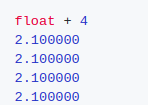
\includegraphics[scale=1.0]{../resources/bon_resultat.png}
\end{block}
\end{frame}

\begin{frame}{Vectorisation}
\begin{block}{sous test 2 / : l'appel des probes vectorielles}
\begin{itemize}
        \item\textit {Nous avons généré le fichier intermédiaire pendant la compilation avec la commande : \textbf{\color{blue} –save-temps }
        \item\textit{une foit le fichier généré , on remarque que on a effectivement fait appel à notre probe vectorielle}} 
        

        \end{itemize}
\end{block}
\begin{block}{exemple}
  \centering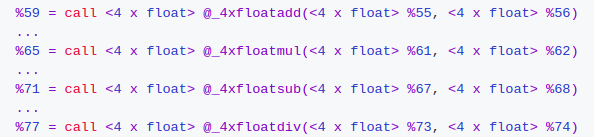
\includegraphics[scale=0.5]{../resources/appel_des_fonction.png}
\end{block}


  
        
\end{frame}

\begin{frame}{Vectorisation}   

\begin{block}{sous test3 / :Utilisation des jeux d’instructions vectorielles}
     \begin{itemize}
     \item\textit{Dans verificarle, les instructions vectorielles pour les opérations arithmetiques sont présentées par la concaténation de  : operation,vectoriel,précision } 
      \item\textit{elle s'utilise sur les registres \textbf{xmm,ymm,zmm } associés respectivement au jeux d'instructions \textbf{sse,avx,avx512} } 
      
   \end{itemize}
  \end{block}
  \begin{block}{exemple}
  \centering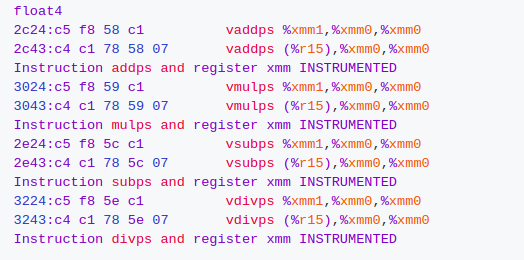
\includegraphics[scale=0.4]{../resources/ajout_instructions.png}
\end{block}
 \end{frame}

\begin{frame}{Vectorisation}         
\begin{block}{support des vecteurs 512/256 bits}
     \begin{itemize}
         \item les vecteurs 256 et 512 bits sont déja inclus et supportés
     \end{itemize}
     
\end{block}
\begin{block}{Ajout des probes vectorielles}
    \begin{itemize}
    \item\textit{les probes vectorielles sont implémentées avec la version scalaire.}
    \item\textit{ajout des fonctions vectorielles pour toutes les operations et mettre la taille des vecteur en paramétre dans les backends}
    \item\textit{Appel des fonction vectorielles des backends dans: \textbf{src/vfcwrapper/main.c} } 
   \end{itemize}  
\end{block}
 \end{frame}

\begin{frame}{Vectorisation}         
\begin{block}{Ajout des fonctions vectorielles des backends dans l’interface}
  \begin{itemize}
  \item\textit{ajouter dans l'interface qui se trouve dans le fichier \textbf{src/common/interflop.h}} 
 
 \item\textit{Comme nous passons la taille en argument, il faudra tester la taille pour permettre à clang d’effectuer une opération vectorielle en changeant le type de notre tableau dans le bon type vectorielles de clang.}
 \item\textit{changer le type vectorielles en son pointeur sur sa précision.}
 \item\textit{Deplacer la définitions des types vectorielles dans le fichier src/common/inteflop.h .}
   \end{itemize}
    
\end{block}
\end{frame}

\begin{frame}{Vectorisation}
    \begin{block}{Récapitulatif}
      \begin{figure}
          \centering
          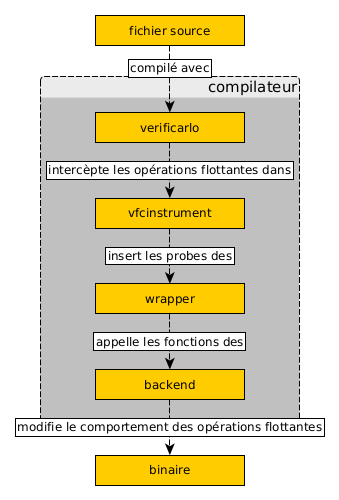
\includegraphics[scale=0.3]{../ressources/verificarlo_works.png}
          \caption{Fonctionnement de verificarlo}
          \label{fig:fonctionnement_verificarlo}
      \end{figure}
    \end{block}
\end{frame}

\begin{frame}{Changements aux niveaux des backends}

  \begin{block}{Backend existant}
    \begin{itemize}
    \item backend ieee
    \item backend vprec
    \item backend mca
    \item backend bitmask
    \item backend cancellation
    \item backend mca-mpfr
    \end{itemize}
  \end{block}

  \begin{block}{Fonctions vectorielles en mode scalaire}
    \begin{itemize}
    \item mode par défaut
    \item tous les backends
    \end{itemize}
  \end{block}

  \begin{block}{Fonctions vectorielles en mode vectoriel}
    \begin{itemize}
    \item backend ieee
    \item backend vprec
    \end{itemize}
  \end{block}

\end{frame}

\begin{frame}{Changements aux niveaux du backend vprec}

  \begin{block}{Fonctionnement du backend}
    \begin{itemize}
    \item norme IEEE754
    \item fonction de débogue
    \end{itemize}
  \end{block}

  \begin{block}{Opérandes constantes}
    \begin{itemize}
    \item avertissement de clang sur les types des paramètres de fonction
    \item ajout d'un pragma pour retirer l'avertissement
    \end{itemize}
  \end{block}

\end{frame}

\begin{frame}{Changements aux niveaux du backend vprec}

  \begin{block}{Fonctionnement du backend}
    \begin{itemize}
    \item nombres fini et infini
    \item nombres normaux et dénormaux
    \end{itemize}
  \end{block}

  \begin{figure}
    \centering
    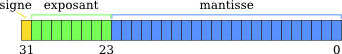
\includegraphics[width=200px]{../ressources/IEEE754_simple_precision.png}
    \caption{\label{fig:ieee_simple_precision}Représentation d'un nombre flottant simple précision}
  \end{figure}

\end{frame}

\begin{frame}{Compilation}

  \begin{block}{Ajout à la compilation de Verificarlo}
    Compilation des \textbf{wrappers} et des \textbf{backends} avec le drapeau:
    \begin{center}
      \textbf{-march=native}
    \end{center}
  \end{block}

  \begin{block}{Avantage}
    Détection automatique des jeux d'instructions disponnibles
  \end{block}


\end{frame}

\begin{frame}{Problèmes rencontrés}

  \begin{block}{Jeu d'instruction disponnible}
    SSE
  \end{block}

  \begin{block}{Types vectorielles}
    Vecteur de 4 double précision = 256 bits
  \end{block}

  \begin{block}{Clang}
    Utilise 4 addition vectoriel SSE
  \end{block}

  \begin{block}{Verificarlo}
    \begin{itemize}
    \item Backend: vectorisé comme pour clang
    \item Problème: vecteur passé par registre entre les modules
    \end{itemize}
  \end{block}

\end{frame}

\begin{frame}{Conclusion}

  \begin{block}{Fait}
    \begin{itemize}
    \item test opérations vectorielles simple
    \item probes vectorielles
    \item fonctions vectorielles (mode scalaire ou vectoriel)
    \item activation des jeux d'instruction
    \end{itemize}
  \end{block}

  \begin{alertblock}{Reste à faire}
    \begin{itemize}
    \item test des conditions vectorielles
    \item test des opérations vectorielles spécifique aux backends
    \item vectorisé les backends manquants
    \item test des performances
    \end{itemize}
  \end{alertblock}

  \begin{block}{Cours en relation}
    Architecture Parallèle
  \end{block}

\end{frame}

\end{document}
